\documentclass[tikz,border=10pt]{standalone}
\begin{document}
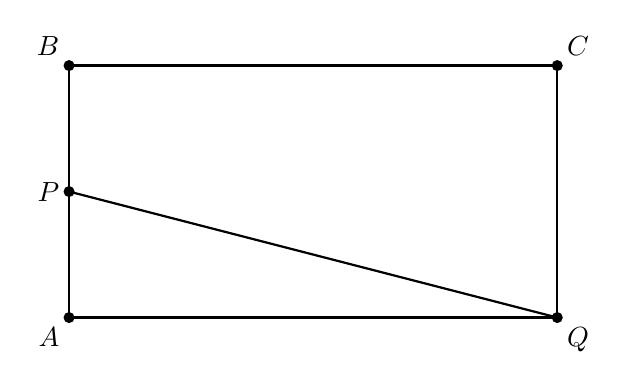
\begin{tikzpicture}[line cap=round,line join=round]

\coordinate (A) at (0,0);
\coordinate (B) at (0,3.2);
\coordinate (C) at (6.2,3.2);
\coordinate (Q) at (6.2,0);
\coordinate (P) at (0,1.6);

\draw[thick] (A) -- (B) -- (C) -- (Q) -- (A);
\draw[thick] (P) -- (Q);

\fill (A) circle (2pt);
\fill (B) circle (2pt);
\fill (C) circle (2pt);
\fill (P) circle (2pt);
\fill (Q) circle (2pt);

\node[below left] at (A) {$A$};
\node[above left] at (B) {$B$};
\node[above right] at (C) {$C$};
\node[left] at (P) {$P$};
\node[below right] at (Q) {$Q$};

\end{tikzpicture}
\end{document}
